When working with level sets you almost always work with small objects
in a much bigger context. This is due to the fact that our level set
is defined in on a Cartesian grid, and we have to manipulate all grid
cells(from here on referred to as the workspace) to make sure the SDF
is always welldefined, meaning the length of the gradient is equal to
one. This is a time consuming process as described in
section \vref{sec:reinitialize}. A solution to make the processes
faster is to only work on the area of the SDF just beside the contour
of interest. This method is called the narrow band method and is
described in \cit{adalsteinsson1995fast}. A narrow band of the Aarhus
University(AU) logo can be seen in figure \vref{fig:nb-au-logo} where (a)
shows the input figure given to the program, and (b) showing the
narrow band generated from the interface of the input.


\begin{figure}[h]
  \centering
  \subfloat[The input]{
    
\includegraphics[width=0.3\textwidth]{imgs/nb-au}}
  \subfloat[The Narrow band]{
    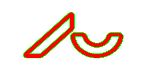
\includegraphics[width=0.3\textwidth]{imgs/nb-au-band}}

  \caption{Visualizing the narrow band of the AU logo.}
  \label{fig:nb-au-logo}
\end{figure}

\section{Idea of the Narrow Band Method}
The basic idea of the method is to narrow down the amount of grid
cells we are working on, to include as few as possible without loosing
accuracy. This is done by keeping a band of $\gamma$ calls around the
interface so we only update the SDF only where
$-\gamma \leq \phi(x,y) \leq \gamma$. When we solve the level set
equation within the narrow band, we use the values of the neighboring
cells. On the edge of the band we cannot be sure the values of their
neighbors are valid as they aren't in the narrow band, and this is
where the outer band, also called an safety band, comes in to
play. All the neighbors on both sides of our narrow band is added to
this set. The only job of the outer band is to supply the inner band
with information when calculating on the border of the band. Because
we know how big $\gamma$ is, it is safe to assume that the distance
from the outer band to $\phi=0$ is more or less $\gamma$. Setting the
value of all cells in the outer band to $\gamma$ is therefore safe if
we promise to reinitialize the band, after solving the level set
equation, to make the length of the gradients one.  This will make the
whole narrow band including the outer band satisfy the requirements of
the SDF and we only have to reinitialize inside the band itself. Hence
the program flow is changed a little. We first evolve the interface by
solving the level set equation on the SDF. We then recalibrate the
narrow band to fit the newly generated SDF and then at the end
reinitialize inside the narrow band.


\begin{figure}[!ht]
  \centering
  \begin{tabular}{ | c | }
   \hline			
   Solve level set equation \\
   \hline
   Update narrow band \\
   \hline   
   Reinitialize \\
   \hline  
  \end{tabular}
  \caption{Program flow with narrow band}
  \label{fig:narrowband_flow}
\end{figure}


To decide the size of $\gamma$, and thereby the width of the narrow
band, we have to look at the maximum distance the interface can move
in a time step. In our implementation this boundary is at one cell
per time step, therefore a narrow band of size 3 around the interface
is sufficient. As seen in figure \vref{fig:nb-au-logo} the band
reaches just outside the interface border as displayed in red. The
green outline around the red band is the outer safety band.

\begin{figure}[h]
  \centering 
  \subfloat[The output]{ 
  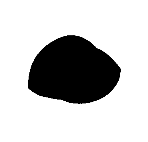
\includegraphics[width=0.3\textwidth]{imgs/nb1}} 
  \subfloat[Without narrow band]{ 
  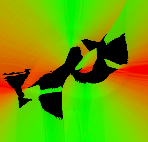
\includegraphics[width=0.3\textwidth]{imgs/nb2}} 
  \subfloat[With narrow band]{ 
  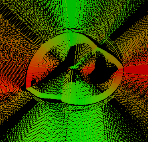
\includegraphics[width=0.3\textwidth]{imgs/nb3}} 

  \caption{A morph between two figures (AU-logo to a circle) showing
  the gradient map with and without the narrow band method. In the
  gradient map we have also shown places where the length of the
  gradient is different from zero, here depicted with the color
  black.}

 \label{fig:narrowBand}
\end{figure}

As seen in figure \vref{fig:narrowBand}, the narrow band method is
powerful. Using the method we have significantly lowered the number of
grid cells needed to visit while working with the SDF, simultaneously we
have reduced the number of times needed to reinitialize. If we only
reinitialize once it is clear that the method without narrow band is
more correct overall, though it contains large amounts of wrong data
around the interface, making calculations faulty. The narrow band
version is clearly wrong in the majority of the cells, but around the
interface we see that the narrow band is in effect and the one
reinitialisation per time step almost covers our needs. 


\section{Implementation}
To represent our Narrow band we need a data structure to hold the new
information. Normally we traverse the workspace linearly and know
which cells have been updated, and which we are going to visit
next. In the narrow band approach we have no linearity and, the narrow
band can be divided into many detached objects in the
workspace. Therefore we need another way to traverse it than run
through (x,y) in the height and width of the workspace. Our solution is
to keep every grid cell in a vector with (x,y) coordinates, and append the
vectors of the cells inside the narrow band to a list. This list will
then contain the complete narrow band, both inner and outer band. To
distinguish the two bands from each other we are using a two dimensional matrix
holding a 1 if the said cell is in the inner band, and a 2 if it is
in the outer, 0 means the cell is in neither. We also maintain an
integer containing the number of cells inside the narrow band.

To build the narrow band, the technique is simply to traverse the SDF
and check the distance to an interface. If we are within the $\gamma$
range of it, we are inside the narrow band, and the cell is added to
the set of cells inside the band. Simultaneously  we add the said cell to
the matrix telling which of the bands it is contained in. For
simplicity we can in the same traversal check if it should be in the
outer band if it isn't inside the inner band. As it does not matter if
we take too much in the outer band, we here just check if it is in
$\gamma$ range + 2 cells. We take more than needed, but we are on the
safe side. The type of the cells in the outer band is of course added
to the type matrix. This is done as shown by this code:
%\todoVester{Omformuler}
%\subsection{Building the initial narrow band}
\begin{lstlisting}
    for (unsigned int x=0; x<width; x++)
        for (unsigned int y=0; y<height; y++) {
            float phiVal = fabs((*phi)(x, y));
            if (phiVal <= narrowBandWidth) {
                //Part of the inner band
                narrowBand[narrowBandSize++] = (Vector<2,int> (x,y));
                nbType(x,y) = 1;
            } else if (phiVal <= narrowBandWidth + 2.0f) {
                //Part of the outer(safety) band
                narrowBand[narrowBandSize++] = (Vector<2,int> (x,y));
                nbType(x,y) = 2;
            } else {
                nbType(x,y) = 0;
            }
        }
\end{lstlisting}


%% \section{Rebuilding the narrow band}
%% \todoVester{3 linjer der forklarer hvad man gør}
%% As we have defined a narrow band to work inside, it seems odd to
%% rebuild this every time step by traversing the entire
%% workspace. In \cit{peng1999pde} is described a solution where the
%% rebuilding time of the narrow band has been optimized. We again use
%% the fact that we know our interface only can move 1 cell per time step,
%% hence our new inner band must be within the old narrow band. Knowing
%% this we only need to traverse the old narrow band to see which cells
%% are within $\gamma$ distance of our new interface position. Whilst
%% doing this we also update the type matrix, removing the cells which no
%% longer reside inside a band. Now the tricky part comes; finding the
%% outer band. This can be done in a separate step, where we traverse the
%% new inner band, and for each cell visits the neighbors. If the
%% neighbor is set to 0 in the type matrix, we change it to 2, and add it
%% to the end of our narrow band list. Many of the visited cells will
%% already be inside the narrow band, but the time spared not traversing
%% the entire workspace is worth it. 


                %% if ((*phi)(x,y) >= 0)
                %%     (*phi)(x,y) =peng1999pde narrowBandWidth;
                %% else 
                %%     (*phi)(x,y) = -narrowBandWidth;



\section{Discussion}
%\todoVester[inline]{Skriv NB Conclution} 

Testing the narrow band method we got an significant speedup. We did
not get to implement a faster version for rebuilding the narrow band
as explained in \cit{peng1999pde}. In this version of the narrow
band they rebuild the narrow band inside the old narrow band. This can
be done as the interface only moves one cell per time step. Therefore
we can build the new inner band inside the old narrow band. The new
outer band can then be found be traversing the neighbors of the new
inner band. 

%The next step of our implementation of the narrow band method will be
%to integrate it with CUDA, hoping to obtain even faster run times.



%%% Local Variables: 
%%% mode: latex
%%% mode: auto-fill
%%% TeX-PDF-mode: t
%%% TeX-master: "../master.tex"
%%% End: 
